% =============================================================================
% Block 9 --- Aula 9: AS-AD policy (Benigno 2015, sections 6-12). Notation: see Block 8. Checks: practice-all-topics-check-b.py, Block 9.
% Solution format (rules/00_estilo_avaliacao.md §4): Notation list, numbered equations cited with \eqref,
% one operation per displayed line. Labels: b9q<question>:<name>; AD/AS are \eqref{b8:AD}, \eqref{b8:AS}.
\bloco{9}{AS--AD policy: shocks, divine coincidence, optimal policy, multipliers, ZLB}{Benigno (2015) \S\S6--12 (Aula 9) \,\textbullet\, 25 points}

\questao{(5 points) Objective items.}

\textbf{a)} (3 points) Which shock leaves the central bank a trade-off between $p=p^e$ and $y=y_e$, and why?
\begin{alternativas}
\item A temporary rise in the current markup $\mu$: it lowers $y_n$ but not $y_e$, so $p=p^e$ and $y=y_e$ cannot both hold on the AS.
\item A temporary rise in productivity $a$: it lowers $p$ along the AD, so a cut in $i$ cannot bring $p$ back to $p^e$ without a gap.
\item News of a higher long-run markup $\bar\mu$: it shifts the AS up today and separates $y_n$ from $y_e$ in the current period.
\item News of higher long-run productivity $\bar a$: it lifts demand above $y_e$, and raising $i$ lowers $p$ but leaves a positive gap.
\end{alternativas}
\gabarito{A}
\begin{sol}
\begin{notacao}
\item $y_n$, $y_e$: natural and efficient output; $\mu$, $\bar\mu$: current and long-run markups; $a$, $\bar a$: productivity; $y_n'$: natural output after the shock.
\end{notacao}
\passo{key}{Efficient output is natural output \eqref{b8q22:yn} without the markup:}
\begin{equation}
y_e=\frac{(1+\eta)a+\sigma^{-1}g}{\sigma^{-1}+\eta}. \label{b9q25:ye}
\end{equation}
Subtracting \eqref{b9q25:ye} from \eqref{b8q22:yn}:
\begin{align}
y_n-y_e&=\Big(\frac{(1+\eta)a+\sigma^{-1}g-\mu}{\sigma^{-1}+\eta}\Big)-\Big(\frac{(1+\eta)a+\sigma^{-1}g}{\sigma^{-1}+\eta}\Big)\nonumber\\
&=-\frac{\mu}{\sigma^{-1}+\eta}, \label{b9q25:gap}
\end{align}
which depends on the current markup only. After $\mu\uparrow$ the AS \eqref{b8:AS} passes through $(y_n',p^e)$ with $y_n'<y_e$:
on it, $p=p^e$ means $y=y_n'\neq y_e$. Since $i$ moves only the AD, the bank picks a point on that AS; none gives both.
\passo{distractors}{B: by \eqref{b9q25:gap}, $a$ moves $y_n$ and $y_e$ together, so a cut in $i$ restores $p=p^e$ \emph{and} $y=y_n=y_e$ (\S6.1). C makes two mistakes:
$\bar\mu$ moves the AD, not the AS, and it leaves current $y_n=y_e$ (so the bank offsets it fully). D: raising $i$ by $d\bar y_n/\sigma$ returns
the AD to $E$, closing price and output gaps at once (\S6.3).}
\refbib{Benigno (2015), \S6--\S7, Figs.~6--9, pp.~511--514; \S11, p.~522.}
\end{sol}

\medskip
\textbf{b)} (2 points, T or F) A temporary rise in the labor-income tax $\tau$ (with $i$, $\bar p$, $p^e$ fixed) lowers output and also lowers
the output gap $y-y_n$.
\gabarito{F}
\begin{sol}
\begin{notacao}
\item $\tau$: labor-income tax (part of $\mu$); $D\equiv(\sigma^{-1}+\eta)(1+\sigma\kappa)>0$ (defined below); $\kappa>0$: AS slope.
\end{notacao}
\passo{proof}{Differentiate \eqref{b8:AD} with $\bar y_n$, $g$, $i$, $\bar p$ fixed, and \eqref{b8:AS} with $p^e$ fixed:}
\begin{equation}
dy=-\sigma\,dp,\qquad dp=\kappa(dy-dy_n). \label{b9q25:dADAS}
\end{equation}
Substitute the second equation of \eqref{b9q25:dADAS} into the first and solve for $dy$:
\begin{align}
dy&=-\sigma\big(\kappa(dy-dy_n)\big)\nonumber\\
dy&=\frac{\sigma\kappa\,dy_n}{1+\sigma\kappa}. \label{b9q25:dy}
\end{align}
By \eqref{b8q22:yn}, with $d\mu=d\tau$,
\begin{equation}
dy_n=-\frac{d\tau}{\sigma^{-1}+\eta}. \label{b9q25:dyn}
\end{equation}
Substitute \eqref{b9q25:dyn} into \eqref{b9q25:dy}, with $D\equiv(\sigma^{-1}+\eta)(1+\sigma\kappa)$:
\begin{align}
dy&=\frac{\sigma\kappa\,\big(-\frac{d\tau}{\sigma^{-1}+\eta}\big)}{1+\sigma\kappa}\nonumber\\
\frac{dy}{d\tau}&=-\frac{\kappa\sigma}{D}<0. \label{b9q25:dydtau}
\end{align}
Subtract \eqref{b9q25:dyn} from \eqref{b9q25:dydtau}, writing $\frac1{\sigma^{-1}+\eta}=\frac{1+\sigma\kappa}{D}$:
\begin{align*}
\frac{d(y-y_n)}{d\tau}&=-\frac{\kappa\sigma}{D}+\frac{1+\sigma\kappa}{D}\\
&=\frac1D>0 .
\end{align*}
The tax cuts $y_n$ by more than it cuts $y$, so the gap rises.
\refbib{Benigno (2015), \S8, eqs.~(22)--(23), Table~1, pp.~514--515.}
\end{sol}

% -----------------------------------------------------------------------------
\questao{(8 points) \textit{Source: built on Benigno, P. (2015), ``New-Keynesian Economics: An AS--AD View'', \S8, pp.~514--516
--- the article has no exercises; the statement below is ours.}
The spending multiplier: Benigno's eqs.~(22)--(23), Tables~1--2. Take $i=\rho$, $\bar p=p^e=0$, $a=\mu=0$, and a temporary rise in
$g$ with $\bar g$ fixed.}

\noindent What the article states (p.~514): ``In particular, an increase in current public expenditure, $g\uparrow$, increases output.
The increase is one-to-one in the special case of linear disutility of labor, i.e.\ $\eta=0$; otherwise the increase is less than
proportional.''

\textbf{a)} (3 points) Derive the output multiplier $m_g=dy/dg$ from the AD and AS curves. Show that $m_g\le1$, with equality iff $\eta=0$.
\resolespaco
\begin{sol}
\begin{notacao}
\item $g$, $\bar g$: government spending today and in the long run (log deviations); $m_g=dy/dg$: output multiplier.
\item $\sigma>0$, $\eta\ge0$, $\kappa>0$ as in Block 8; $D\equiv(\sigma^{-1}+\eta)(1+\sigma\kappa)$.
\end{notacao}
\passo{setup}{With $i=\rho$, $\bar p=p^e=0$ and no consumption taxes, \eqref{b8:AD} and \eqref{b8:AS} become}
\begin{align}
y&=\bar y_n+(g-\bar g)-\sigma[(\rho)-((0)-p)-(0)-\rho]\nonumber\\
y&=\bar y_n+g-\bar g-\sigma p, \label{b9q26:AD}\\
p-(0)&=\kappa(y-y_n)\nonumber\\
p&=\kappa(y-y_n), \label{b9q26:AS}
\end{align}
and \eqref{b8q22:yn} with $a=\mu=0$ gives
\begin{align}
y_n&=\frac{(1+\eta)(0)+\sigma^{-1}g-(0)}{\sigma^{-1}+\eta}\nonumber\\
&=\frac{\sigma^{-1}g}{\sigma^{-1}+\eta}. \label{b9q26:yn}
\end{align}
Substitute \eqref{b9q26:AS} into \eqref{b9q26:AD}:
\begin{align}
y&=\bar y_n+g-\bar g-\sigma\big(\kappa(y-y_n)\big)\nonumber\\
y&=\bar y_n+g-\bar g-\sigma\kappa y+\sigma\kappa y_n\nonumber\\
(1+\sigma\kappa)\,y&=g+\bar y_n-\bar g+\sigma\kappa\,y_n. \label{b9q26:comb}
\end{align}
\passo{multiplier}{In \eqref{b9q26:comb}, $g$ enters directly ($+1$) and through $y_n$; by \eqref{b9q26:yn} the second channel is
$\sigma\kappa\cdot\frac{\sigma^{-1}}{\sigma^{-1}+\eta}=\frac{\kappa}{\sigma^{-1}+\eta}$. Differentiating \eqref{b9q26:comb} with respect to $g$:}
\begin{align}
(1+\sigma\kappa)\,m_g&=1+\sigma\kappa\Big(\frac{\sigma^{-1}}{\sigma^{-1}+\eta}\Big)\nonumber\\
m_g&=\frac{1+\frac{\kappa}{\sigma^{-1}+\eta}}{1+\sigma\kappa}\nonumber\\
&=\frac{\sigma^{-1}+\eta+\kappa}{D}. \label{b9q26:mg}
\end{align}
\passo{bound}{From the first line of \eqref{b9q26:mg}:}
\begin{align*}
m_g\le1&\iff1+\frac{\kappa}{\sigma^{-1}+\eta}\le1+\sigma\kappa\\
&\iff\frac1{\sigma^{-1}+\eta}\le\sigma\\
&\iff1\le1+\sigma\eta\\
&\iff\eta\ge0 .
\end{align*}
Equivalently, since $D=\sigma^{-1}+\eta+\kappa+\sigma\kappa\eta$, the second line of \eqref{b9q26:mg} gives
\begin{align}
1-m_g&=1-\Big(\frac{\sigma^{-1}+\eta+\kappa}{D}\Big)\nonumber\\
&=\frac{(\sigma^{-1}+\eta+\kappa+\sigma\kappa\eta)-(\sigma^{-1}+\eta+\kappa)}{D}\nonumber\\
&=\frac{\sigma\kappa\eta}{D}, \label{b9q26:1mg}
\end{align}
zero iff $\eta=0$. With $\eta>0$, spending raises prices and the real rate, crowding out consumption.
\rubrica{\item AD and AS combined: 1 pt. \item $m_g$ with both channels: 1 pt. \item Bound with the iff: 1 pt.}
\end{sol}

\textbf{b)} (3 points) Find the multiplier on the gap $y-y_n$ and on the efficient gap $y-y_e$. Why are they so much smaller than $m_g$?
\resolespaco
\begin{sol}
\begin{notacao}
\item Symbols as in (a); $y_e$: efficient output \eqref{b9q25:ye}.
\end{notacao}
\passo{gap}{By \eqref{b9q26:yn}, $dy_n/dg=\frac{\sigma^{-1}}{\sigma^{-1}+\eta}$. Over the common denominator $D$,}
\begin{equation}
\frac{\sigma^{-1}}{\sigma^{-1}+\eta}=\frac{\sigma^{-1}(1+\sigma\kappa)}{D}=\frac{\sigma^{-1}+\kappa}{D}. \label{b9q26:ynD}
\end{equation}
Subtract \eqref{b9q26:ynD} from \eqref{b9q26:mg}:
\begin{align}
\frac{d(y-y_n)}{dg}&=\frac{\sigma^{-1}+\eta+\kappa-(\sigma^{-1}+\kappa)}{D}\nonumber\\
&=\frac{\eta}{D}. \label{b9q26:gapm}
\end{align}
By \eqref{b9q25:ye}, $y_e$ has the same $g$-coefficient as $y_n$ in \eqref{b8q22:yn}, so the multiplier on $y-y_e$ is also $\frac\eta D$.
\passo{why}{Most of the extra output is supply: public spending makes households poorer, so they work more and $y_n$ rises,
by \eqref{b9q26:yn} (Benigno's eq.~15). Only the part of $y$ above the new $y_n$ is a demand effect, and that is what the gap measures.}
\rubrica{\item Gap multiplier derived: 1.5 pts. \item Same for $y-y_e$, with the reason: 0.5 pt. \item Interpretation: 1 pt.}
\end{sol}

\textbf{c)} (2 points) Evaluate $\kappa$, $m_g$, the gap multiplier and $1-m_g$ at the calibration, and compare with Table~2.
\resolespaco
\begin{sol}
\begin{notacao}
\item $\alpha=0.66$: share of preset prices; $\sigma=0.5$, $\eta=0.2$, $\sigma^{-1}+\eta=2.2$ (Block 8 calibration).
\end{notacao}
\passo{numbers}{Using $\kappa=\frac{(1-\alpha)(\sigma^{-1}+\eta)}{\alpha}$, then $D$, \eqref{b9q26:mg}, \eqref{b9q26:gapm} and \eqref{b9q26:1mg}:}
\begin{align*}
\kappa&=\frac{0.34\times2.2}{0.66}=1.133,\\
1+\sigma\kappa&=1+0.5\times(1.133)\\
&=1.567,\qquad D=2.2\times1.567=3.447,\\
m_g&=\frac{2.2+1.133}{3.447}=0.967,\\
\frac{\eta}{D}&=\frac{0.2}{3.447}=0.058,\\
1-m_g&=\frac{0.5\times1.133\times0.2}{3.447}=0.033 .
\end{align*}
Table~2 prints $0.96$ for $m_g$ in this row.
\refbib{Confirmed against Benigno (2015), Table~2, p.~516, and the project's Map note on Benigno \S8 (note 07: 0.967 and 0.058).}
\rubrica{\item Each of $\kappa$, $m_g$, gap: 0.5 pt; comparison: 0.5 pt.}
\end{sol}

% -----------------------------------------------------------------------------
\questao{(12 points) Discursive. \emph{The Copom's three meetings.} Start from the efficient steady state: $y_n=y_e=0$,
$p^e=\bar p=0$, $i=\rho=2\%$. The welfare loss is $L=\frac12(y-y_e)^2+\frac{\theta}{2\kappa}(p-p^e)^2$ (eq.~33) with $\theta=8$; use the calibration of
Block~8 and work in percentage points.}

\textbf{a)} (4 points) Meeting 1: news that long-run productivity will rise, $d\bar a=1$, current $a$ unchanged (say, gains from
agricultural technology expected to last). Which curves move? Find $y$ and $p$ if the bank keeps $i=\rho$, and the optimal $i$.
Is there a trade-off? Contrast with a temporary rise in $a$.
\resolespaco
\begin{sol}
\begin{notacao}
\item $y$, $p$: output and price level; $y_n$, $y_e$: natural and efficient output; $\bar y_n$: long-run natural output; $p^e=\bar p=0$.
\item $a$, $\bar a$: current and long-run productivity; $i$: policy rate; $\rho=2\%$: rate of time preference.
\item $r_n$: natural rate of interest, the $i$ that sets $y=y_n$ at $p=p^e$ (defined in step 3); $E$: the initial equilibrium.
\item $L$: welfare loss; $\theta=8$: weight on price surprises; $\kappa=1.133$, $\sigma=0.5$, $\eta=0.2$.
\end{notacao}
\passo{curves}{Differentiate \eqref{b8q22:ybn} with respect to $\bar a$:}
\begin{align*}
d\bar y_n&=\frac{(1+\eta)\,d\bar a}{\sigma^{-1}+\eta}\\
&=\frac{(1+0.2)\times(1)}{2.2}=\frac{1.2}{2.2}=0.545 .
\end{align*}
Households expect to be richer and consume more now, so by \eqref{b8:AD} the AD shifts right by $0.545$. $y_n$ \eqref{b8q22:yn} and $y_e$
\eqref{b9q25:ye} depend on current $a$, so AS does not move.
\passo{no policy}{The algebra of Block 8, \eqref{b8q24:dy} and \eqref{b8q24:dAS}, applies with $d\bar y_n=0.545$:}
\begin{align*}
dy&=\frac{d\bar y_n}{1+\sigma\kappa}=\frac{0.545}{1.567}=0.348,\\
dp&=\kappa\,dy\\
&=1.133\times(0.348)=0.395 .
\end{align*}
Output is above both $y_n$ and $y_e$, prices above $p^e$.
\passo{policy}{With $p=\bar p$, $g=\bar g$ and no consumption taxes, \eqref{b8:AD} reads $y=\bar y_n-\sigma(i-\rho)$. Setting $y=y_n$ and solving for $i$:}
\begin{align}
(y_n)&=\bar y_n-\sigma(r_n-\rho)\nonumber\\
r_n&=\rho+\sigma^{-1}(\bar y_n-y_n). \label{b9q27:rn}
\end{align}
By \eqref{b9q27:rn}, $r_n$ rises by $0.545/0.5=1.09$ points. Setting $i=r_n$, i.e.\ \emph{raising} $i$ to $3.09\%$, returns the AD to $E$:
$y=y_n=y_e$, $p=p^e$, $L=0$. No trade-off (divine coincidence): $y_n=y_e$ throughout. A temporary $a\uparrow$ is the mirror image:
the AS shifts right, the AD stays, and the bank must \emph{cut} $i$; a permanent one needs no change.
\rubrica{\item Curve identification: 1 pt. \item No-policy equilibrium: 1 pt. \item Policy sign and size, no trade-off: 1.5 pts.
\item Contrast: 0.5 pt. Moving the AS for news, or cutting $i$: max.\ 1 pt in the item.}
\end{sol}

\textbf{b)} (5 points) Meeting 2: a temporary markup shock $\mu=5$ (say, a fuel-tax rise), $\bar\mu=0$. Find the outcome at $i=\rho$. Then
minimize $L$ subject to the AS and derive the targeting rule, $y^\ast$, $p^\ast$, and the rate $i^\ast$, comparing it with $r_n$ and $\rho$. Draw.
\resolespaco
\begin{sol}
\begin{notacao}
\item Symbols as in (a); $\mu=5$: current markup shock; $y^\ast$, $p^\ast$, $i^\ast$: optimal output, price level and rate; $E'$: no-policy point; $O$: optimum.
\end{notacao}
\passo{shock}{By \eqref{b8q22:yn} and \eqref{b9q25:ye} with $a=g=0$:}
\begin{align*}
y_n&=\frac{(1+0.2)(0)+0.5^{-1}(0)-(5)}{2.2}\\
&=-\frac{5}{2.2}=-2.273,\qquad y_e=0 .
\end{align*}
AS shifts up through $(y_n,p^e)$; AD unchanged. At $i=\rho$, with $\bar y_n=g=\bar p=p^e=0$, \eqref{b8:AD} and \eqref{b8:AS} are
\begin{equation}
y=-\sigma p,\qquad p=\kappa(y-y_n). \label{b9q27:ADAS}
\end{equation}
Substitute the second equation of \eqref{b9q27:ADAS} into the first and solve for $y$; then use the first for $p$:
\begin{align*}
y&=-\sigma\big(\kappa(y-y_n)\big)\\
y&=\frac{\sigma\kappa\,y_n}{1+\sigma\kappa}=\frac{0.567\times(-2.273)}{1.567}=-0.822,\\
p&=-y/\sigma\\
&=-(-0.822)/0.5=1.644 .
\end{align*}
Output falls and prices rise: stagflation.
\passo{why along AS}{$i$ moves only the AD, so the bank chooses \emph{which point of the AS} the economy occupies. The loss of the statement is}
\begin{equation}
L=\tfrac12(y-y_e)^2+\frac{\theta}{2\kappa}(p-p^e)^2. \label{b9q27:L}
\end{equation}
Substitute \eqref{b8:AS}, $p-p^e=\kappa(y-y_n)$, and $y_e=0$ into \eqref{b9q27:L}:
\begin{align}
L(y)&=\tfrac12\big(y-(0)\big)^2+\frac{\theta}{2\kappa}\big(\kappa(y-y_n)\big)^2\nonumber\\
&=\tfrac12y^2+\frac{\theta\kappa}2(y-y_n)^2. \label{b9q27:Ly}
\end{align}
Differentiate \eqref{b9q27:Ly} and set it to zero (the second derivative is $1+\theta\kappa>0$):
\begin{equation}
y+\theta\kappa(y-y_n)=0. \label{b9q27:foc}
\end{equation}
Since $\kappa(y-y_n)=p-p^e$ by \eqref{b8:AS}, and $y_e=0$, \eqref{b9q27:foc} is the targeting rule
\begin{align}
y+\theta\big(p-p^e\big)&=0\nonumber\\
(y-y_e)+\theta(p-p^e)&=0. \label{b9q27:IT}
\end{align}
\passo{optimum}{Solve \eqref{b9q27:foc} for $y$; then subtract $y_n$ and use \eqref{b8:AS}:}
\begin{align}
y^\ast&=\frac{\theta\kappa\,y_n}{1+\theta\kappa}\nonumber\\
&=\frac{8\times1.133\times(-2.273)}{1+8\times1.133}\nonumber\\
&=\frac{9.067}{10.067}(-2.273)=-2.047, \label{b9q27:ystar}\\
p^\ast&=\kappa(y^\ast-y_n)\nonumber\\
&=\kappa\Big(\Big(\frac{\theta\kappa\,y_n}{1+\theta\kappa}\Big)-y_n\Big)\nonumber\\
&=-\frac{\kappa y_n}{1+\theta\kappa}=\frac{1.133\times2.273}{10.067}=0.256. \label{b9q27:pstar}
\end{align}
\passo{rate}{With $\bar y_n=g=\bar p=0$, \eqref{b8:AD} reads}
\begin{equation}
y=-\sigma(i+p-\rho). \label{b9q27:ADi}
\end{equation}
Solve \eqref{b9q27:ADi} for $i$ at \eqref{b9q27:ystar}--\eqref{b9q27:pstar}:
\begin{align*}
i^\ast&=\rho-p^\ast-y^\ast/\sigma\\
&=2-(0.256)-(-2.047)/0.5\\
&=2-0.256+4.094=5.838\% .
\end{align*}
By \eqref{b9q27:rn} with $\bar y_n=0$, the natural rate is
\begin{align*}
r_n&=\rho+\sigma^{-1}\big((0)-y_n\big)\\
&=2-\frac{(-5/2.2)}{0.5}=6.545\%.
\end{align*}
So $\rho<i^\ast<r_n$: the bank tightens, accepting a deeper fall in output to keep prices close to $p^e$, but it accommodates part of
the shock. By \eqref{b9q27:ystar}--\eqref{b9q27:pstar}, as $\theta\to\infty$, $y^\ast\to y_n$ and $p^\ast\to p^e$ (strict price stability); as $\theta\to0$, $y^\ast\to y_e$.
\begin{center}
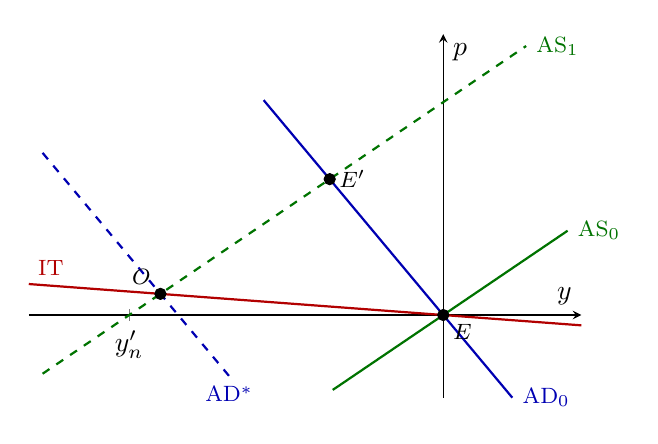
\begin{tikzpicture}
\begin{axis}[width=8.6cm,height=6.2cm,xmin=-3,xmax=1,ymin=-1,ymax=3.4,xlabel={$y$},ylabel={$p$},axis lines=middle,
  xtick={-2.273},xticklabels={$y_n'$},ytick=\empty,clip=false]
\addplot[green!45!black,thick,domain=-0.8:0.9] {1.133*x} node[right] {\footnotesize AS$_0$};
\addplot[green!45!black,thick,dashed,domain=-2.9:0.6] {1.133*(x+2.273)} node[right] {\footnotesize AS$_1$};
\addplot[blue!70!black,thick,domain=-1.3:0.5] {-2*x} node[right] {\footnotesize AD$_0$};
\addplot[blue!70!black,thick,dashed,domain=-2.9:-1.55] {0.256-2*(x+2.047)} node[below] {\footnotesize AD$^\ast$};
\addplot[red!70!black,thick,domain=-3:1] {-x/8} node[pos=0.04,above] {\footnotesize IT};
\addplot[only marks,mark=*] coordinates {(0,0) (-0.822,1.644) (-2.047,0.256)};
\node[below right] at (axis cs:0,0) {\footnotesize $E$};
\node[right] at (axis cs:-0.822,1.644) {\footnotesize $E'$};
\node[above left] at (axis cs:-2.047,0.256) {\footnotesize $O$};
\end{axis}
\end{tikzpicture}
\end{center}
\refbib{Confirmed against the Lista~7 answer in \emph{Map}, \texttt{lista-07.md}: no policy $(-0.82,+1.64)$; optimum $y^o=-2.05$, $p^o=+0.26$,
$i^o=5.84\%$ vs $r_n=6.55\%$. Benigno (2015), \S7 and \S11, eq.~(33), Fig.~14, pp.~513--514 and 521--523.}
\rubrica{\item Shock and no-policy point: 1 pt. \item Loss minimized \emph{along AS} with the reason: 1.5 pts (differentiating in $i$ with AD as the
constraint: max.\ 0.5). \item $y^\ast$, $p^\ast$, targeting rule: 1 pt. \item $i^\ast$ vs $r_n$, $\rho$, and $\theta$ limits: 0.5 pt. \item Graph with IT line and $O$: 1 pt.}
\end{sol}

\textbf{c)} (3 points) Meeting 3: news that long-run productivity will fall, $d\bar a=-5$, with $\mu=a=0$. Show that the required rate is
negative. With $i=0$, find the gap and $p$. What can the bank still do, and on what does it depend?
\resolespaco
\begin{sol}
\begin{notacao}
\item Symbols as in (a); ZLB: the zero lower bound $i\ge0$; $\bar p-p^e$: the long-run price level the bank promises, relative to preset prices.
\end{notacao}
\passo{required rate}{By \eqref{b8q22:ybn}, $\bar y_n=0.545\times(-5)=-2.727$, while $y_n=0$. By \eqref{b9q27:rn}:}
\begin{align*}
r_n&=\rho+\sigma^{-1}\big(\bar y_n-(0)\big)\\
&=2+\frac{(-2.727)}{0.5}=2-5.455=-3.455\%<0 .
\end{align*}
Cash pays zero, so $i\ge0$: the ZLB binds.
\passo{at $i=0$}{Substitute \eqref{b8:AS} into \eqref{b8:AD} (with $g=\bar g$, no consumption taxes), subtract $y_n$ and use \eqref{b9q27:rn}:}
\begin{align}
y&=\bar y_n-\sigma\big[i-\big(\bar p-(p^e+\kappa(y-y_n))\big)-\rho\big]\nonumber\\
(1+\sigma\kappa)(y-y_n)&=(\bar y_n-y_n)-\sigma\big[i-(\bar p-p^e)-\rho\big]\nonumber\\
(1+\sigma\kappa)(y-y_n)&=\big(\sigma(r_n-\rho)\big)-\sigma\big[i-(\bar p-p^e)-\rho\big]\nonumber\\
y-y_n&=\frac{\sigma}{1+\sigma\kappa}\left[r_n-i+(\bar p-p^e)\right]. \label{b9q27:gapz}
\end{align}
At $i=0$ and $\bar p=p^e$, \eqref{b9q27:gapz} and \eqref{b8:AS} give
\begin{align*}
y-y_n&=\frac{0.5}{1.567}\big[(-3.455)-(0)+(0)\big]\\
&=\frac{0.5}{1.567}(-3.455)=-1.103,\\
p-p^e&=\kappa(y-y_n)\\
&=1.133\times(-1.103)=-1.250 .
\end{align*}
\passo{expectations}{By \eqref{b9q27:gapz}, the gap closes at $i=0$ if the bank commits to a higher long-run price level,
$\bar p-p^e=-r_n=3.455$. Higher expected inflation $\bar p-p$ lowers the real rate when the nominal rate cannot fall. It works only if
the promise is credible (the bank must tolerate the higher $\bar p$ later).}
\rubrica{\item $r_n<0$: 1 pt. \item Gap and $p$ at $i=0$: 1 pt. \item The $\bar p$ commitment, its size and credibility: 1 pt.}
\end{sol}
